\chapter{Introduction}

\section{Présentation du sujet}
Le module \emph{Initiation à la recherche} du 2\up{nd} semestre du master \textsc{ALMA} propose une initiation au métier de chercheur en informatique. Dans le cadre de ce module notre binôme a choisi le sujet : \emph{Conception et réalisation d’un logiciel interactif de visualisation de pavages 2D/3D}. Ce sujet à la particularité d'être la reprise d'un projet de stage. Ce stage effectué au cours de l'été 2011 par un membre du binôme avait pour objectif initial la conception réalisation d'un outil de visualisation des calculs en sortie du logiciel  \realpaver (cf. \ref{realp}) développé au sein de l'équipe d'accueil. Le développement de ce stage a suivit le modèle du cycle en V décrit par la figure \ref{fig:vcycle}.
\begin{figure}[htbp]
\centering
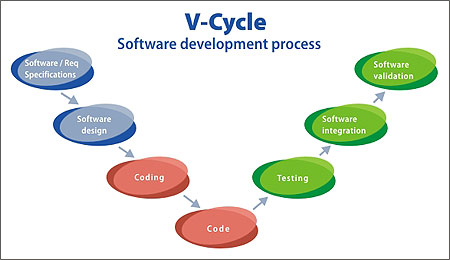
\includegraphics[scale=1]{img/vcycle}
\caption{Cycle en V}
\label{fig:vcycle}
\end{figure}
\clearpage
Au terme des deux mois de stage, le travail accompli fut le suivant :
\begin{enumerate}
\item 
Rédaction du cahier des charges (cf. \ref{sec:cac}).
\item
Rédaction du document de spécification (cf. \ref{sec:spe}).
\end{enumerate} 

\section{\'Equipe d'accueil}
L'\'Equipe \textsc{OPTI} Optimisation globale, optimisation multi-objectifs\cite{opti} du laboratoire \textsc{LINA}\cite{lina} travaille principalement sur des méthodes visant à la résolution efficace de problèmes d’optimisation complexes.  
\section{Déroulement du projet}
Au cours des premières semaines, C.\textsc{Jermann} nous a proposé d'étudier de manières générales les sujets de l'équipe \textsc{OPTI}. Un bref bilan de cette étude est proposé dans le chapitre \ref{chap:doc}. En parallèle, nous avons manipulé quelques outils ad-hoc que gnuplot \cite{gnu}, utilisés jusqu'à présent par l'équipe \textsc{OPTI} pour représenter les valuations calculées par \realpaver. Par la suite nous avons pris (ou repris) connaissances du cahier des charges et du documents de spécifications, en apportant certaines correction à ce dernier.  \\
Une problématique est apparue quant à l'axe d'étude à choisir par la suite. En effet une des caractéristiques principale de l'outil à concevoir, est de manipuler un nombre potentiellement très grands de données (cf. \ref{chap:con}). Nos alternatives étaient alors les suivantes : 
\begin{enumerate}
\item
Etudier les différents algorithmes et structures de données nécessaires à l'outil.
\item
Entamer directement la conception de l'outil (choix de design pattern, IHM, \dots).
\end{enumerate} 
Ce second choix impliquait la possibilité au terme de l'année, de proposer un résultat «materiel». En effet le document de spécifications étant très concis, nous aurions pu très rapidement produire du code en le suivant à la lettre. Cependant cette démarche ne répondait pas aux objectifs de découverte du module d'Initiation à la Recherche. De plus, passez outre cette étude de structures et d'algorithmes, aurait rapidement entraîné la conception dans une impasse. Nous avons donc choisi la seconde alternative. Notre contribution à cette étude est résumé dans le chapitre \ref{chap:con} de ce document.

